% !TEX root = _individual/flatland.tex

%%%%%%%%%%%%%%%%%%%%%%%%%%%%%%%%%%%%%%%%%%%%%%%%%%%%%%%%%%%%%%%%%%%%%%%%%%%%%%%%
\chapter{Flatland Geometry}\label{chap:flatland}

Flatland geometry is a fictional space where particles are
constrained to travel in a two-dimensional plane \cite{Abb1884,Asa2008}. This
differs from standard 2-D
geometry, which is a slice of a 3-D problem that is invariant in the $z$ axis.
Because the flatland phase space is
$(x,y,\theta)$ with \emph{one} angular variable $\theta$, rather than the
standard 2D $(x,y,\mu,\theta)$ with \emph{two} angular variables $\mu$ and
$\theta$, flatland is a computationally simpler testing ground that retains the
complexity of multidimensional geometry. For this reason, flatland has recently
been used in the development and testing of multi-D transport methods
\cite{Lar2009c,Joh2011,Tra2011}.

To briefly illustrate the difference between flatland and 2-D geometry, we
view an infinite gap between two materials. The flatland problem and the
two-dimensional projection are identical, shown in Fig.~\ref{fig:chordFlatland}.
%
\begin{figure}[htb]
  \centering
  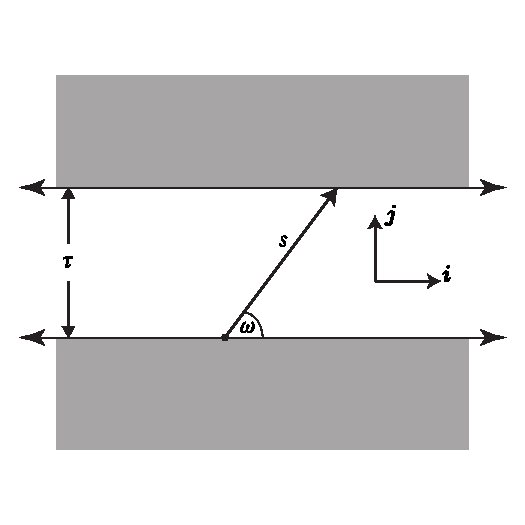
\includegraphics{chord-flatland}
  \caption[The infinite gap as represented on paper.]%
  {The infinite gap as represented on paper. The gap is a distance
  $\tau$ across, $\theta$ is the azimuthal angle, and $s$ is the
  distance across the gap.}
  \label{fig:chordFlatland}
\end{figure}
%
However, in the 2-D case, the figure is merely a slice of a three-dimensional
problem where the two gray rectangles and the gap are infinite in extent
(Fig.~\ref{fig:chordXy}).
%
\begin{figure}[htb]
  \centering
  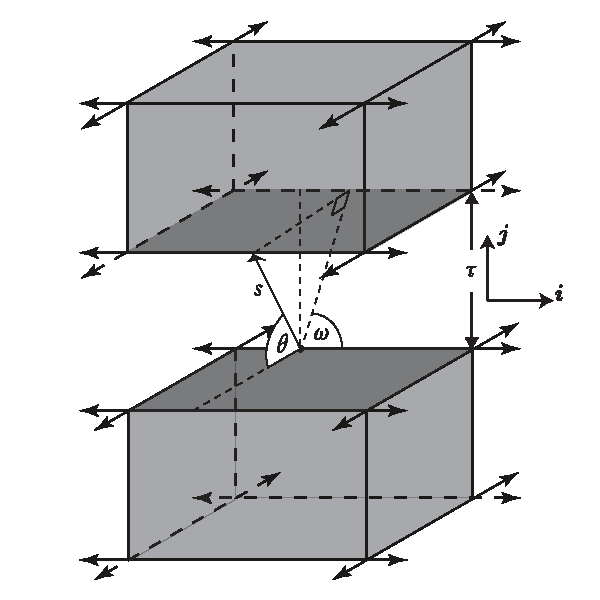
\includegraphics{chord-xyz}
  \caption[A fuller view of the infinite gap in 2-D geometry.]%
  {A fuller view of the infinite gap in 2-D geometry.
  The polar angle cosine is $\mu= \cos \varphi$, and the azimuthal angle is
  $\theta$.}
  \label{fig:chordXy}
\end{figure}

%For the purposes of comparison, we also consider Fig.~\ref{fig:chordFlatland} as
%a sagittal view of an infinite cylinder; Fig.~\ref{fig:chordRz} shows a
%cross-sectional view.
%
%\begin{figure}[htb]
%  \centering
%  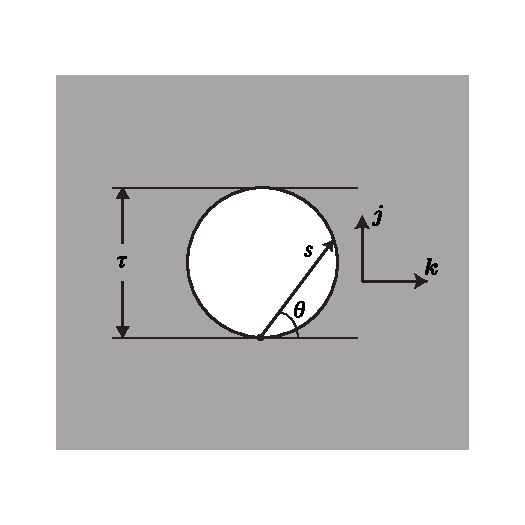
\includegraphics{chord-rz}
%  \caption[A cross-section of the chord length problem in cylindrical
%  geometry.]%
%  {A cross-section of the chord length problem in cylindrical
%  geometry. The orthogonal view looks like Fig.~\ref{fig:chordFlatland}.}
%  \label{fig:chordRz}
%\end{figure}

Despite being easier computationally to solve, flatland has a few subtle quirks.
For example, previous work in flatland \cite{Asa2008,Lar2009c} has shown that the
diffusion coefficient for flatland geometry $\frac{1}{2\sigma}$ is different
from the physical diffusion coefficients $\frac{1}{3\sigma}$, but accurate
boundary conditions for the flatland diffusion equations have not been derived.
We also present Monte Carlo sampling algorithms tailored to flatland
geometry, as well as a quick description of how 2-D \SN\ transport can easily be
adapted to flatland.

These methods are implemented in flatland primarily for the purpose of
comparison with the new anisotropic diffusion methods. We briefly derive the
AD approximation in flatland geometry for use in our benchmark problems.

%%%%%%%%%%%%%%%%%%%%%%%%%%%%%%%%%%%%%%%%%%%%%%%%%%%%%%%%%%%%%%%%%%%%%%%%%%%%%%%%
\clearpage
\section{Transport in flatland}

The flatland transport equation describes particle emission, absorption, and
movement in the flatland geometry.
Because the time-dependent and nonlinear terms of thermal radiative transfer are
not affected by the choice of geometry, we constrain our discussion in this
section to a steady-state problem. Furthermore, the behavior of specular
reflection is identical in any geometry, so we only take the case of a specified
incident boundary condition. Our application of the flatland transport equation
has only isotropic emission (and ``pseudo-scattering'' if the linearized
transport equation is used), so we limit our study to the case of isotropic
scattering.

To begin, we write the steady-state transport equation with isotropic scattering
in a new ``general geometry'' form valid both for flatland and real space (1-D,
2-D,
and 3-D):
\begin{subequations} \label{eqs:ssTransport}
\begin{equation}\label{eq:ssTransportVol}
  \vec{\Omega}\vd \grad I(\vec{x}, \vec{\Omega})
  + \sigma(\vec{x}) I(\vec{x}, \vec{\Omega})
  = \frac{1}{\omega_0} \phi(\vec{x}) \,,
  \quad \vec{x} \in V \,,\ \vec{\Omega} \in \Omega\,.
\end{equation}
Here, we use
\begin{align*}
  I(\vec{x},\vec{\Omega}) &= \text{the steady-state angular intensity,} \\
  \vec{\Omega} &= \text{the angular variable,} \\
  \Omega &= \text{the domain of the angular variable (the ``unit sphere''),} \\
  \omega_n &= \text{the $n$th angular moment, and} \\
  \phi(\vec{x}) &= \text{the scalar intensity, the zeroth angular moment of $I$.}
\end{align*}
The angular variables $\vec{\Omega}$ and domains $\Omega$ are defined in
Table~\ref{tab:angularDomain}, and the moments $\omega_0$ are evaluated in
Table~\ref{tab:angularMoments}. The specified incident radiation
boundary:
\begin{equation} \label{eq:ssBndy}
  I(\vec{x}, \vec{\Omega}) = I^b(\vec{x}, \vec{\Omega})
  \quad \vec{x} \in \partial V \,,\ \vec{\Omega} \vd \vec{n} < 0\,.
\end{equation}
\end{subequations}

\begin{table}[htb]
  \centering
  \begin{tabular}{rccc}
\toprule
   Geometry & $\vec{\Omega}$ & Domain $\Omega$ & $\ud\Omega$
\\ \midrule
   1-D & $\mu$ & $-1 \le \mu \le 1$ & $\ud\mu$
   \\
   2-D & $\sqrt{1-\mu^2} \cos \theta \vec{i}
   + \sqrt{1-\mu^2} \sin \theta \vec{j}$
   & $-1 \le \mu \le 1$, $0 \le \theta < 2\pi$ & $\ud\mu \ud \theta$
   \\
   Flatland & $\cos \theta \vec{i} + \sin \theta \vec{j}$
   & $0 \le \theta < 2\pi$ & $\ud \theta$
   \\
   3-D & $\mu \vec{i}
   + \sqrt{1-\mu^2} \cos \theta \vec{j}
   + \sqrt{1-\mu^2} \sin \theta \vec{k}$
   & $-1 \le \mu \le 1$, $0 \le \theta < 2\pi$ & $\ud\mu \ud \theta$
\\ \bottomrule
  \end{tabular}
  \caption{Angular variables in the various geometries.}
  \label{tab:angularDomain}
\end{table}

\begin{table}[htb]
  \centering
  \begin{tabular}{rccc}
\toprule
   Geometry
   & $\omega_0 \equiv \int_\Omega \ud\Omega$
   & $\omega_1 \equiv \int_\Omega \abs{\vec{\Omega}\vd\vec{i}} \ud\Omega$
   & $\omega_2 \equiv \int_\Omega (\vec{\Omega}\vd\vec{i})^2 \ud\Omega$
\\ \midrule
   1-D & 2 & 1 & $\frac{2}{3}$
   \\
   2-D & $4\pi$ & $2\pi$ & $\frac{4\pi}{3}$
   \\
   Flatland & $2\pi$ & $4$ & $\pi$
   \\
   3-D & $4\pi$ & $2\pi$ & $\frac{4\pi}{3}$
\\ \bottomrule
  \end{tabular}
  \caption{Angular moments in each geometry.}
  \label{tab:angularMoments}
\end{table}

The so-called ``unit sphere''---%
the domain of the angular variable $\vec{\Omega}$---%
differs among the geometries. In 3-D, $\norm{\vec{\Omega}}=1$, so valid angles
lie on the surface of a sphere of unit radius. In 2-D, those angles are
projected onto a slice through the sphere's middle, so that
$\norm{\vec{\Omega}} \le 1$: valid angles are on a unit disc. Angles on the edge
of the disc---the unit circle---represent particles traveling along the slice,
and angles inside the unit circle are the projection of 3-D angles traveling with a
non-zero polar angle cosine. Flatland geometry allows only angles on the unit
circle, $\norm{\vec{\Omega}}=1$.

%%%%%%%%%%%%%%%%%%%%%%%%%%%%%%%%%%%%%%%%
\subsection{Monte Carlo sampling}

In testing the anisotropic diffusion approximation, we use the Monte Carlo
method to generate the reference solutions.
The Monte Carlo method approximates the transport equation by tracking the
random lives of statistically large numbers of particles as they traverse a
problem. The behavior during their lifetime depends on probability distribution
functions (PDFs) that describe how they are born, how far they travel without a
collision, how they behave when they collide, and so on.

The general Monte Carlo process has been covered extensively elsewhere
\cite{Lew1984,Bro2004a}; our focus in this section is to expound upon the
distributions particular to flatland geometry.
We briefly derive those PDFs,
integrate them to get cumulative distribution functions
(CDFs), and use the direct inversion method to show how a uniformly sampled
pseudo-random number $\xi \in [0,1)$ may be used to determine particle behavior
in flatland. Because the geometry tracking routines of steady state Monte Carlo
and Fleck and Cummings' IMC are identical, the results in this section are
applicable any flatland Monte Carlo implementation.

\subsubsection{Isotropic volume source}
A particle emitted from an isotropic internal source, whether an extraneous
radiation source or an indirect isotropic scattering event, has an equal
probability of entering any angle. In any geometry, the normalized PDF that
represents this process is
\begin{equation}\label{eq:volumeSource1}
  f(\vec{\Omega}) \ud \Omega = \alpha \ud \Omega \,,
  \quad \vec{\Omega} \in \Omega \,,
\end{equation}
where (see Table~\ref{tab:angularDomain}) $\Omega$ is the angular domain of the
geometry and $\alpha$ is a normalization constant.
Requiring the PDF to integrate to unity over its domain gives the
following value for $\alpha$ in any geometry:
\begin{align*}
  1 = \int_{\Omega} f(\vec{\Omega}) \ud\Omega
  = \alpha \int_{\Omega} \ud\Omega
  \lra
  \alpha = \frac{1}{\omega_0}\,.
\end{align*}
Thus the angular distribution of an isotropic volume source is
\begin{equation}\label{eq:volumeSource2}
  f(\vec{\Omega}) \ud \Omega = \frac{\ud\Omega}{\omega_0} \,,
  \quad \vec{\Omega} \in \Omega\,.
\end{equation}

In 2-D, using the identities from Tables~\ref{tab:angularDomain}
and~\ref{tab:angularMoments}, Eq.~\eqref{eq:volumeSource2} evaluates to the
familiar
\begin{equation*}
  f(\mu,\theta) \ud\mu\ud\theta = \frac{\ud\mu\ud\theta}{4\pi} 
  = \frac{\ud\mu}{2}\frac{\ud\theta}{2\pi}
  \,,
  \quad -1\le \mu \le 1,\ 0 \le \theta < 2\pi\,,
\end{equation*}
which gives the separable CDF
\begin{equation*}
  F(\mu,\theta) = F_1(\mu) F_2(\theta)
  = \frac{1 + \mu}{2}\frac{\theta}{2\pi}\,,
  \quad -1\le \mu \le 1,\ 0 \le \theta < 2\pi\,.
\end{equation*}
Setting two uniformly sampled random numbers $\xi_1 = F(\mu)$ and
$\xi_2 = F(\theta)$, solving for $\mu$ and $\theta$, and
introducing them back into the 2-D representation of $\vec{\Omega}$, we get the
well-known result
\begin{align*}
  \vec{\Omega} &= \sqrt{1-\mu^2} \cos \theta \vec{i}
  + \sqrt{1-\mu^2} \sin \theta \vec{j}
\\
  &= \sqrt{1-(2\xi_1-1)^2} \cos(2\pi\xi_2) \vec{i}
  + \sqrt{1-(2\xi_1-1)^2} \sin(2\pi\xi_2) \vec{j}\,.
\end{align*}

In flatland, Eq.~\eqref{eq:volumeSource2} becomes the simpler
\begin{equation*}
  f(\theta) \ud\theta = \frac{\ud\theta}{2\pi} \,,
  \quad 0 \le \theta < 2\pi\,,
\end{equation*}
yielding the CDF
\begin{equation}\label{eq:volumeSourceFlatland}
  F(\theta) = \frac{\theta}{2\pi}\,,
  \quad 0 \le \theta < 2\pi\,,
\end{equation}
Setting $\xi_1 = F(\theta)$ and solving for $\theta = F\inv(\xi_1)$ gives the
following simple relation between an isotropically sampled angle $\theta$ and a
uniformly sampled random number $\xi_1$:
\begin{equation*}
  \theta = 2\pi \xi_1\,.
\end{equation*}
The flatland particle's new angle is therefore
\begin{equation*}
  \vec{\Omega} = \cos \theta \vec{i} + \sin \theta \vec{j}
  = \cos(2\pi\xi_1) \vec{i} + \sin(2\pi\xi_1) \vec{j}\,.
\end{equation*}

With only one independent variable that needs sampling, and the omission of
the transcendental operation $\sqrt{1-\mu^2}$, the computational cost of a
scattering event is less in flatland than in 2-D, leading to
faster simulation times.

\subsubsection{Isotropic surface source}\label{sec:isoSurface}
Particles emitted from an isotropic surface source have a cosine distribution
\cite{Gre2002}, which has a constant radiation flux in each differential
angle:
\begin{equation}\label{eq:surfaceSource1}
  f(\vec{\Omega}) \ud \Omega = \alpha \abs{\vec{\Omega}\vd \vec{n}} \ud \Omega \,,
\quad \vec{\Omega}\vd \vec{n} < 0 \,,
\end{equation}
where $\alpha$ is a normalization constant.
Requiring the PDF to integrate to unity over its domain gives $\alpha$
\begin{align*}
  1 &= \int_{\vec{\Omega}\vd \vec{n} < 0} \left[ \alpha \abs{\vec{\Omega}\vd
  \vec{n}} \right] \ud\Omega
  \\
  1 &=\frac{\alpha}{2} \int_{\Omega} \abs{\vec{\Omega}\vd \vec{n}} \ud\Omega
  \\
  \alpha &= \frac{2}{\omega_1}\,,
\end{align*}
so that the PDF for an isotropic surface source,
Eq.~\eqref{eq:surfaceSource1}, becomes
\begin{equation}\label{eq:surfaceSource2}
  f(\vec{\Omega}) \ud \Omega = \frac{2}{\omega_1} \abs{\vec{\Omega}\vd \vec{n}} \ud \Omega \,,
\quad \vec{\Omega}\vd \vec{n} < 0 \,.
\end{equation}

In 3-D, choosing $\vec{n}=\vec{i}$, the isotropic surface PDF is
\begin{equation*}
  f(\mu,\theta) \ud\mu \ud\theta
  = \frac{1}{\pi} \mu \ud\mu \ud\theta
  = (2 \mu \ud\mu) \frac{\ud\theta}{2\pi}\,,
\end{equation*}
which gives the separable CDF
\begin{equation*}
  F(\mu,\theta) = (\mu^2) \frac{\theta}{2\pi}\,,
\end{equation*}
from which we can sample $\mu=\sqrt{\xi_1}$ and $\theta=2\pi \xi_2$.

In flatland, the surface source distribution is different. Let us choose
$\vec{n} = -\vec{j}$ so that incident directions are in the range
$\theta \in [0, \pi)$.
Using the flatland identities in Tables~\ref{tab:angularDomain}
and~\ref{tab:angularMoments} to Eq.~\eqref{eq:surfaceSource1} gives the surface
source PDF of
\begin{equation*}
  f(\theta) \ud\theta = \frac{2}{4} \, \abs{ -\sin \theta}\ud\theta
  = \frac{1}{2} \sin \theta\ud\theta \,,\quad 0 \le \theta < \pi\,.
\end{equation*}
Integrating, we obtain the CDF for particle emission from
a surface source in flatland geometry:
\begin{equation}\label{eq:surfaceSourceFlatland}
  F(\theta) = \frac{1}{2} \left( 1-\cos\theta \right)
  \,,\quad 0 \le \theta < \pi\,,
\end{equation}
Solving for $\theta = F\inv(\xi_1)$ gives a sampled angle for a surface source
in flatland:
\begin{equation*}
  \theta = \cos\inv(1 - 2\xi_1)\,.
\end{equation*}
Finally, we insert this into the flatland $\vec{\Omega}$ and use the identity
$\cos^2 \theta + \sin^2 \theta = 1$ to reduce the number of transcendental
functions. The direction of a particle from an isotropic surface source is
\begin{align*}
  \vec{\Omega} &= \cos \theta \vec{i} + \sin \theta \vec{j} \\
  &=  \cos[ \cos\inv(1 - 2\xi_1) ] \vec{i} + \sin[ \cos\inv(1 - 2\xi_1) ] \vec{j} \\
  &= (1 - 2\xi_1) \vec{i} + \sqrt{1 - (1 - 2\xi_1)^2} \vec{j}\,.
\end{align*}

%%%%%%%%%%%%%%%%%%%%%%%%%%%%%%%%%%%%%%%%
\subsection{Discrete ordinates quadrature}

A standard practice in two-dimensional discrete ordinates (\SN) solvers is to
create a quadrature set that only creates polar angles for the top half of a
unit sphere, $\mu>0$, and to modify the ordinate weights to sum to $4\pi$
\cite{Zik1997}. A properly designed quadrature set will also approach the 2-D
moments of Table~\ref{tab:angularMoments} as the number of ordinates
$N$ in the quadrature approaches infinity:
\begin{equation*}
  \omega_n \approx \sum_{m=1}^{N} w_m \abs{ \vec{\Omega}_m \vd \vec{i}}^n \,.
\end{equation*}

The most straightforward way of implementing the flatland geometry in an \SN\
code with only isotropic scattering is to create a special quadrature set
consisting of ordinates that have a single
polar angle $\mu=0$. To retain compatibility with the isotropic scattering
kernel, the quadrature weights are normalized so that they sum to $4\pi$
instead of $2\pi$. This way, none of the discrete ordinates logic has to be
modified: all of the angular moments
\begin{equation*}
  \phi_n(\vec{x}) \approx \sum_{m=1}^{N} w_m \vec{\Omega}_m^n I_m
\end{equation*}
will give correct flatland answers. Thus an anisotropic diffusion tensor $\Dtens$
will be calculated in flatland just as in 2-D geometry.

This scaling has two notable side effects. First, because the weights are twice
what they should be, the \SN\ angular moments approach twice the flatland
moments $\omega_n$:
\begin{equation*}
  2 \omega_n \approx \sum_{m=1}^{N} w_m \abs{ \vec{\Omega}_m \vd \vec{i}}^n \,.
\end{equation*}
Also, with this approach, visualizing $I(\theta)$ by plotting
$I_m$ as a function of $\theta_m$ requires multiplying by a factor of two.
% Here is an
%example that uses the \verb|matplotlib| Python module's polar plot to view
%the flatland angular intensity:
%\begin{verbatim}
%    polar( [ angle.getPhi() for angle in quadrature_set ],
%           [ 2 * value for value in psi ] )
%\end{verbatim}

%%%%%%%%%%%%%%%%%%%%%%%%%%%%%%%%%%%%%%%%%%%%%%%%%%%%%%%%%%%%%%%%%%%%%%%%%%%%%%%%
\section{Diffusion in flatland}

An accurate diffusion formulation
is imperative for benchmarking the anisotropic diffusion
approximation against diffusion solutions.
The angular moments in Table~\ref{tab:angularMoments},
\begin{equation*}
  \omega_n \equiv \int_\Omega \abs{\vec{\Omega} \vd \vec{i}}^n \ud \Omega\,,
\end{equation*}
determine the constants in the diffusion coefficient and boundary conditions.
Previous work has given the flatland diffusion coefficient to be $1/2\sigma$,
and in the following section we derive ``Marshak'' and ``variational'' boundary
conditions for the flatland diffusion equation. (We published a summary of
our work in \cite{Joh2011a}.)
%There is no loss of generality in
%ignoring the time dependence because of the quasi-static approximation made in
%the derivation of the diffusion coefficient (see \S\ref{sec:bgDiffusion}).

%%%%%%%%%%%%%%%%%%%%%%%%%%%%%%%%%%%%%%%%
\subsection{Interior diffusion approximation}

The diffusion approximation begins by assuming that $I$ is linear in angle:
\begin{equation*}
  I(\vec{x}, \vec{\Omega}) \approx f(\vec{x}) + \vec{\Omega} \vd
  \vec{g}(\vec{x})\,.
\end{equation*}
The zeroth angular moment of $I$ determines $f$:
\begin{equation*}
  \phi = \int_\Omega I \ud \Omega
= \int_\Omega \left( f + \vec{\Omega}\vd \vec{g} \right) \ud\Omega
= \int_\Omega\ud\Omega f + 0
= \omega_0 f \,,
\end{equation*}
and the first moment of $I$ determines $g$:
\begin{equation*}
  \vec{F} = \int_\Omega \vec{\Omega} I \ud \Omega
= f \int_\Omega \vec{\Omega} \ud\Omega
  + \vec{g} \vd \int_\Omega \vec{\Omega}\vec{\Omega} \ud\Omega
= \omega_2 \vec{g} \,.
\end{equation*}
Thus is the \Pone\ approximation to the radiation intensity in ``general
geometry'' form,
\begin{equation}\label{eq:ssPone}
  I(\vec{x}, \vec{\Omega})
  \approx \frac{1}{\omega_0} \phi(\vec{x})
  + \frac{1}{\omega_2} \vec{\Omega} \vd \vec{F}(\vec{x})\,.
\end{equation}

The diffusion approximation is a closure for the first angular moment of
the transport equation, so we now operate on Eq.~\eqref{eq:ssTransportVol} with
$\int_\Omega \vec{\Omega} (\cdot) \ud \Omega$ and substitute
Eq.~\eqref{eq:ssPone}:
\begin{align*}
  \grad \vd \int_\Omega \vec{\Omega} \vec{\Omega} I
  \ud\Omega
  + \sigma \int_\Omega \vec{\Omega} I \ud\Omega
  &= \frac{1}{\omega_0} \phi \int_\Omega \vec{\Omega} \ud\Omega
  \\
  \grad \vd \int_\Omega \vec{\Omega} \vec{\Omega} \left(
  \frac{1}{\omega_0}\phi + \frac{1}{\omega_2} \vec{\Omega} \vd \vec{F}
  \right)
  \ud\Omega
  + \sigma \vec{F}
  &= 0
  \\
  \frac{1}{\omega_0} \grad \vd \int_\Omega \vec{\Omega} \vec{\Omega}
  \ud\Omega\, \phi 
  + \sigma \vec{F} &= 0
  \\
  \frac{\omega_2}{\omega_0} \grad \phi + \sigma \vec{F} &= 0 \,.
\end{align*}
Solving for $\vec{F}$ gives Fick's law, expressed in the general-geometry form:
\begin{equation} \label{eq:fickGeneral}
  \vec{F}(\vec{x})
  = - \frac{\omega_2}{\omega_0} \frac{1}{\sigma(\vec{x})} \grad \phi(\vec{x})
  \equiv -D(\vec{x}) \grad \phi(\vec{x})\,.
\end{equation}
In 2-D and 3-D, $\omega_2/\omega_0 = (4\pi / 3) / (4\pi) = 1/3$; however, in
flatland, $\omega_2/\omega_0 = \pi / (2\pi) = 1/2$. Thus, $D=(3\sigma)\inv$ in
2-D but $D=(2\sigma)\inv$ in flatland.

Substituting Fick's law back into the linear-in-angle approximation,
Eq.~\eqref{eq:ssPone}, gives the diffusion approximation to the angular
intensity:
\begin{align} \nonumber
  I(\vec{x}, \vec{\Omega})
  &\approx \frac{1}{\omega_0} \phi(\vec{x})
  + \frac{1}{\omega_2} \vec{\Omega} \vd \left[ - \frac{\omega_2}{\omega_0}
  \frac{1}{\sigma(\vec{x})} \grad \phi(\vec{x}) \right]
  \\ \label{eq:diffusionIntensity}
  I(\vec{x}, \vec{\Omega})
  &= \frac{1}{\omega_0} \left[ \phi(\vec{x})
  - \frac{1}{\sigma(\vec{x})}
  \vec{\Omega} \vd \grad \phi(\vec{x}) \right] \,.
\end{align}
In normal space this is
\begin{equation*}
 I(\vec{x}, \vec{\Omega})
= \frac{1}{4\pi} \left[ \phi(\vec{x}) - \frac{1}{\sigma(\vec{x})} \vec{\Omega}
\vd \grad \phi(\vec{x}) \right] \,,
\end{equation*}
and in flatland, the diffusion approximation is
\begin{equation}\label{eq:flatlandDiffusion}
 I(\vec{x}, \vec{\Omega})
= \frac{1}{2\pi} \left[ \phi(\vec{x}) - \frac{1}{\sigma(\vec{x})} \vec{\Omega}
\vd \grad \phi(\vec{x}) \right]\,.
\end{equation}

%%%%%%%%%%%%%%%%%%%%%%%%%%%%%%%%%%%%%%%%
\subsection{Marshak boundary condition}
The Marshak boundary condition \cite{Mar1947} preserves the incident radiation
flux (the partial first moment for incoming directions) on the boundary. It is
derived by substituting the approximate diffusion
intensity from Eq.~\eqref{eq:diffusionIntensity} into the boundary condition,
Eq.~\eqref{eq:ssBndy}, multiplying by $\abs{\vec{\Omega}\vd \vec{n}}$, and integrating over
incident directions.
\begin{align*}
\int_{\vec{\Omega}\vd \vec{n} < 0 } \abs{\vec{\Omega}\vd \vec{n}}
I^b \ud\Omega
 &= 
\int_{\vec{\Omega}\vd \vec{n} < 0 } \abs{\vec{\Omega}\vd \vec{n}} 
 \frac{1}{\omega_0} \left[ \phi - \frac{1}{\sigma}
  \vec{\Omega} \vd \grad \phi \right]
  \ud\Omega
\\
F^{-}
&= 
\frac{1}{\omega_0} \phi \left( \int_{\vec{\Omega}\vd \vec{n} < 0 }
\abs{\vec{\Omega}\vd \vec{n}} \ud\Omega \right) 
  - \frac{1}{\omega_0}\frac{1}{\sigma}
  \int_{\vec{\Omega}\vd \vec{n} < 0 } (-\vec{\Omega}\vd \vec{n})
  \vec{\Omega} \ud\Omega  \vd \grad \phi
\\
F^{-}
&=
\frac{1}{\omega_0} \phi \left( \frac{\omega_1}{2} \right) 
  + \frac{1}{\omega_0}\frac{1}{\sigma} \vec{n} \vd
  \int_{\vec{\Omega}\vd \vec{n} < 0 } \vec{\Omega} \vec{\Omega} \ud\Omega
  \vd \grad \phi
\\
F^{-}
&=
\frac{\omega_1}{2\omega_0} \phi
+ \frac{1}{\omega_0}\frac{1}{\sigma} \vec{n} \vd \left( \frac{\omega_2}{2}
\Identitytens \right) \grad \phi
\\
F^{-}
&=
\frac{\omega_1}{2\omega_0} \phi
+ \frac{\omega_2}{2\omega_0}\frac{1}{\sigma} \vec{n} \vd \grad \phi\,.
\end{align*}
Rearranging gives an expression for the Marshak boundary condition for 
\begin{equation} \label{eq:marshak}
\frac{2\omega_0}{\omega_1} F^{-}
=
\phi + \frac{\omega_2}{\omega_1}\frac{1}{\sigma} \vec{n} \vd \grad \phi
\end{equation}

The value
\begin{equation*}
  z_0 \equiv \frac{\omega_2}{\omega_1}
  =
  \begin{cases}
    \frac{2}{3} \approx 0.6667 & \text{1-D, 2-D, 3-D,} \\
    \frac{\pi}{4} \approx 0.7854 & \text{Flatland,}
  \end{cases}
\end{equation*}
is the Marshak extrapolation distance.

Substituting the diffusion coefficient $D$ from Eq.~\eqref{eq:fickGeneral}
formulates the Marshak boundary condition as
\begin{equation*}
\frac{2\omega_0}{\omega_1} F^{-}
= \phi + \frac{\omega_0}{\omega_1} D \vec{n} \vd \grad \phi\,.
\end{equation*}
In 1-D, 2-D, and 3-D geometries, this evaluates to
\begin{equation*}
4 F^{-}
= \phi + 2 D \vec{n} \vd \grad \phi\,,
\end{equation*}
but in flatland it is
\begin{equation}\label{eq:flatlandDiffusionMarshak}
\pi F^{-}
= \phi + \frac{\pi}{2} D \vec{n} \vd \grad \phi\,.
\end{equation}

%%%%%%%%%%%%%%%%%%%%%%%%%%%%%%%%%%%%%%%%
\subsection{Variational boundary condition} \label{sec:varBndy}
It is known that the Marshak boundary condition is heuristic and not consistent with the
true transport boundary condition. A lengthy asymptotic boundary layer
matching analysis \cite{Hab1975} shows that the correct weighting of the
boundary condition is not $\abs{\vec{\Omega}\vd\vec{n}}$ but rather
$W(\abs{\vec{\Omega}\vd\vec{n}})$, where $W$ is related to Chandrasekhar's
$H$-function \cite{Cha1960}:
\begin{equation*}
  W(\mu) = \frac{\sqrt{3}}{2} \mu H(\mu) \,,
\end{equation*}
which gives an extrapolation distance of
\begin{align*}
  z_0 = \frac{\int_{0}^{1} \mu W(\mu) \ud \mu}{\int_{0}^{1} W(\mu) \ud
  \mu} \approx 0.7104\,.
\end{align*}

A variational analysis \cite{Mal1991} has been used to
derive a very accurate approximation to $W$:
\begin{equation*}
W(\mu) \approx \mu + \tfrac{3}{2} \mu^2 \,,
\end{equation*}
which gives the approximate extrapolation distance of
\begin{equation*}
  z_0 = \frac{\int_{0}^{1} \mu (\mu + \tfrac{3}{2} \mu^2 ) \ud
  \mu}{\int_{0}^{1} (\mu + \tfrac{3}{2} \mu^2 ) \ud \mu} 
  = \frac{17}{24} \approx 0.7083 \,.
\end{equation*}
%This variational analysis can be imitated by taking a semi-infinite,
%source-free, purely scattering transport problem, assuming the exiting $I$ is
%constant in angle, and making a particular demand.

Now we repeat that analysis for flatland rather than real space. The first step
is to form a homogeneous, purely scattering transport problem in a
semi-infinite flatland plane. The transport equation~\eqref{eq:ssTransportVol} becomes
\begin{subequations} \label{eqs:flatTransport}
\begin{equation}\label{eq:flatTransportVol}
  \cos \theta \pder{I}{x} + \sin \theta \pder{I}{y} + \sigma I
  = \frac{\sigma}{2\pi} \int_{0}^{2\pi} I \ud \theta'\,,\quad
 -\infty < x < \infty,\ 0 \le y < \infty,\ 0 \le \theta < 2\pi\,.
\end{equation}
It has a uniform incident boundary condition,
\begin{equation}\label{eq:flatTransportBndy}
  I(x, 0, \theta) = I^b(\theta) \,,\quad -\infty < x < \infty,\ 
  0 \le \theta < \pi \,.
\end{equation}
\end{subequations}

Because there is no variation in the boundary condition or $\sigma$ along
the $x$ axis, $\tpder{I}{x}=0$, and Eq.~\eqref{eq:flatTransportVol} becomes the
one-dimensional transport equation 
\begin{equation*}
  \sin \theta \pder{}{y}I(y,\theta) + \sigma I(y,\theta)
  = \frac{\sigma}{2\pi} \int_{0}^{2\pi} I(y,\theta') \ud \theta'\,.
\end{equation*}
which is \emph{not} the 1-D planar geometry transport equation.

We define the $y$ components of the angular moments of $I$ as
\begin{equation} \label{eq:flatPhi}
  \phi_m(y) = \int_{0}^{2\pi} (\vec{\Omega}\vd\vec{j})^m I(y,\theta) \ud\theta
  = \int_{0}^{2\pi} (\sin\theta)^m I(y,\theta) \ud\theta \,.
\end{equation}

As $y\to\infty$, the intensity $I$ will approach a constant $\varphi/2\pi$,
which gives $\phi_0(\infty)=\varphi$. Concordantly, $\phi_1(\infty)=0$.

Operating on the transport equation by $\int_{0}^{2\pi} (\sin\theta)^m (\cdot)
\ud\theta$ gives the $m$th angular moment in the $y$ direction:
\begin{align} \nonumber
  \pder{}{y} \int_{0}^{2\pi} (\sin\theta)^{m+1} I \ud\theta
  + \sigma \int_{0}^{2\pi} (\sin\theta)^{m} I \ud\theta
  &= \frac{\sigma}{2\pi} \int_{0}^{2\pi} I \ud \theta'
  \int_{0}^{2\pi} (\sin\theta)^{m} \ud\theta
  \\ \label{eq:flatMoments}
  \pder{\phi_{m+1}}{y}
  + \sigma \phi_{m}
  &= \frac{\sigma}{2\pi} \phi_{0}
  \int_{0}^{2\pi} (\sin\theta)^{m} \ud\theta\,.
\end{align}
For $m=0$, the conservation equation, Eq.~\eqref{eq:flatMoments} evaluates to
\begin{equation*}
  \pder{\phi_{1}}{y}
  + \sigma \phi_{0}
  = \frac{\sigma}{2\pi} \phi_{0} (2\pi)
  \lra
  \pder{\phi_{1}}{y} = 0\,.
\end{equation*}
That means the radiation flux is a constant, and because $\phi_1(\infty)=0$,
that constant is zero. Physically, a constant $\phi_1$ means that at every
point, the rate of energy being transferred away from the boundary is balanced
by energy moving toward the boundary. This logically follows from the lack of
absorption in the problem: at steady-state, the only means of energy loss is
through exiting the boundary.

Evaluating Eq.~\eqref{eq:flatMoments} for $m=1$ and using the result that
$\phi_{1}=0$, we obtain
\begin{equation*}
  \pder{\phi_{2}}{y}
  + \sigma \phi_{1}
  = \frac{\sigma}{2\pi} \phi_{0} (0)
  \lra
  \pder{\phi_{2}}{y} = 0\,.
\end{equation*}
Thus $\phi_{2}$ is also a constant. As $y\to\infty$, $I\to\varphi/2\pi$, so
\begin{equation*}
  \phi_{2} = \int_{0}^{2\pi} (\sin\theta)^2 \frac{\varphi}{2\pi} \ud\theta
  = \frac{1}{2} \varphi\,.
\end{equation*}
% in 1-D, this would be $\int_{-1}^{1}\mu^2\frac{\varphi}{2} \ud \mu =
% \frac{1}{3} \varphi$.

Now, since $\phi_1=0$, we can add $\alpha \phi_1$ to this equation for any
$\alpha$:
\begin{align*}
 \alpha\phi_1 + \phi_{2} &= \frac{\varphi}{2} \\
 \int_{0}^{2\pi} (\alpha \sin\theta + \sin^2\theta)
 I(y,\theta) \ud\theta
 &= \frac{\varphi}{2}\,.
\end{align*}
At the boundary $y=0$, $I=I^b$ for incident angles $0 \le \theta < \pi$. The
variational analysis makes the reasonable approximation that, to leading order,
the exiting particles are isotropically distributed, $I(0,\theta)=I^\text{out}$.
\begin{equation*}
 \int_{0}^{\pi} (\alpha \sin\theta + \sin^2\theta)
 I^b(\theta) \ud\theta
 + \int_{\pi}^{2\pi} (\alpha \sin\theta + \sin^2\theta)\ud\theta I^\text{out}
 = \frac{\varphi}{2}\,.
\end{equation*}
The value $\alpha=\pi/4$ eliminates the integral over outgoing directions and
directly relates the moments of the incident angular intensity to the
magnitude of the intensity as $y\to\infty$:
\begin{equation}\label{eq:varBoundary}
 \varphi = 2\int_{0}^{\pi} \left( \frac{\pi}{4} \sin\theta + \sin^2\theta \right)
 I^b(\theta) \ud\theta
 \,.
\end{equation}

We wish our boundary condition to preserve the value of
$\varphi$ when the diffusion method is used, so we substitute the diffusion
approximation, Eq.~\eqref{eq:flatlandDiffusion}:
\begin{align*}
 \varphi &= 2\int_{0}^{\pi} \left( \frac{\pi}{4} \sin\theta + \sin^2\theta \right)
 I^b(\theta) \ud\theta
 \\
 &= 
  2\int_{0}^{\pi} \left( \frac{\pi}{4} \sin\theta + \sin^2\theta \right)
 \left( \frac{1}{2\pi} \phi_0 -
  \frac{1}{\sigma} \sin\theta \pder{\phi_0}{y}\right)\ud\theta
\\
 &= 
\frac{1}{2\pi} \int_{0}^{\pi} \left( \frac{\pi}{2} \sin\theta + 2 \sin^2\theta
\right)\ud\theta
 \,\phi_0 -
 \frac{1}{2\pi} \int_{0}^{\pi} \left( \frac{\pi}{2} \sin^2\theta + 2 \sin^3\theta \right)\ud\theta
  \,\frac{1}{\sigma} \pder{\phi_0}{y}
  \\
 &= 
 \frac{1}{2\pi} \left( \frac{\pi}{2} [2] + 2 \frac{\pi}{2}
\right) \phi_0
-
\frac{1}{2\pi} \left( \frac{\pi}{2} \left[ \frac{\pi}{2} \right] + 2 \left[
\frac{4}{3} \right] \right) \frac{1}{\sigma} \pder{\phi_0}{y}
\\
 &= 
  \phi_0
- \left( \frac{\pi}{8} + \frac{4}{3\pi} \right) \frac{1}{\sigma} \pder{\phi_0}{y}
\,.
\end{align*}
This relationship between $\phi$ and its directional gradient yields the same
value for $\varphi$ when using diffusion as the true incident boundary does
using transport, under the condition of a semi-infinite, homogeneous, purely
scattering problem and an isotropic exiting value for $I$. Problems where the
diffusion approximation is valid satisfy that condition to leading order.

In this problem, we chose a boundary surface normal of $\vec{n}=-\vec{j}$. Now
replacing $\sin \theta$ with $-\vec{\Omega}\vd\vec{n}$, we get the general
boundary condition for flatland diffusion,
\begin{equation} \label{eq:flatlandDiffusionVarBc}
\int_{\vec{\Omega}\vd\vec{n} < 0} \left[ \frac{\pi}{2}
\abs{\vec{\Omega}\vd\vec{n}} + 2 (\vec{\Omega}\vd\vec{n})^2 \right]
I^b(\vec{x}, \vec{\Omega}) \ud\Omega
= 
  \phi_0(\vec{x})
  - \left( \frac{\pi}{8} + \frac{4}{3\pi} \right) \frac{1}{\sigma}
  \vec{n}\vd\grad \phi_0(\vec{x})\,.
\end{equation}

%Essentially, we have shown that the flatland equivalent of the $W$ function,
%which we shall call $V$, can be approximated by
%\begin{equation}\label{eq:flatlandVariational}
%  V(\theta)
%  \approx \frac{1}{4}\sin\theta + \frac{1}{\pi} \sin^2\theta \,,\quad
%  0 \le \theta < \pi \,,
%\end{equation}
%which satisfies
%\begin{equation*}
%  \int_{0}^{\pi} V(\theta) \ud\theta= 1
%\end{equation*}
%and gives the extrapolation distance
%\begin{equation*}
%  z = \frac{\int_{0}^{\pi} \sin \theta V(\theta) \ud\theta}{\int_{0}^{\pi}
%  V(\theta) \ud\theta} =  \frac{\pi}{8} + \frac{4}{3\pi} \,.
%\end{equation*}

%%%%%%%%%%%%%%%%%%%%%%%%%%%%%%%%%%%%%%%%%%%%%%%%%%%%%%%%%%%%%%%%%%%%%%%%%%%%%%%%
\section{Anisotropic diffusion in flatland}
The derivation of the anisotropic diffusion method presented in
chapter~\ref{chap:adDerivation} needs little modification to be formulated
in the flatland geometry. The most notable change is in formulating the
low-order boundary conditions.

We begin with a time-dependent transport equation with isotropic scattering,
using the angular moments from Table~\ref{tab:angularMoments}:
\begin{subequations} \label{eqs:flatfullTransport}
\begin{multline} \label{eq:flatfullTransportVol}
  \frac{1}{c} \pder{I}{t}(\vec{x}, \vec{\Omega}, t)
    + \vec{\Omega}\vd \grad I(\vec{x}, \vec{\Omega}, t)
    + \sigmast(\vec{x}) I (\vec{x}, \vec{\Omega}, t)
    \\ = \frac{1}{\omega_0} \sigmast(\vec{x}) ac [T(\vec{x}, t)]^4
    + \frac{1}{\omega_0} q_{r}(\vec{x}, t)
    \equiv \frac{1}{\omega_0} Q(\vec{x}, t) \,,
\\
x \in V,\  0 \le t \le \Delta_t, \ \vec{\Omega} \in \Omega\,.
\end{multline}
We take the case of an incident radiation source on the boundary:
\begin{equation} \label{eq:flatfullTransportBndy}
  I(\vec{x}, \vec{\Omega}, t) = I^b(\vec{x}, \vec{\Omega}, t) \,,
 \quad \vec{x} \in \partial V, \ \vec{\Omega} \vd \vec{n} < 0,
 \ 0 \le t \le \Delta_t\,.
\end{equation}
The intensity has the initial condition
\begin{equation} \label{eq:flatfullTransportInit}
 I(\vec{x}, \vec{\Omega}, 0) = I^i(\vec{x}, \vec{\Omega}) \,,
 \quad \vec{x} \in V, \ \vec{\Omega} \in \Omega\,,
\end{equation}
which is usually the solution from the previous time step.
\end{subequations}
For the sake of simplicity, we do not consider reflecting boundaries, as their
formulation is identical to the previous derivation of the AD approximation.

Operating on Eq.~\eqref{eq:flatfullTransportVol} by $\int_{\Omega} (\cdot) \ud
\Omega$ gives the radiation energy conservation equation,
\begin{subequations} \label{eqs:flatloEquations}
\begin{equation} \label{eq:flatloVol}
\frac{1}{c} \pder{\phi}{t} (\vec{x}, t)
  + \grad \vd\vec{F}(\vec{x}, t)
  + \sigmast(\vec{x}) \phi(\vec{x}, t)
  = \sigmast(\vec{x}) ac [T(\vec{x}, t)]^4 + q_{r}(\vec{x}, t)
  = Q(\vec{x}, t)\,,
\end{equation}
for $\vec{x} \in V$ and $0 \le t \le \Delta_t$.
Doing the same to the initial condition, Eq.~\eqref{eq:flatfullTransportInit}, gives 
\begin{equation} \label{eq:flatloInit}
\phi(\vec{x}, 0) = \int_{\Omega}  I^i(\vec{x},
\vec{\Omega}) \ud\Omega = \phi^i(\vec{x})\,, \qquad \vec{x} \in V  \,.
\end{equation}
\end{subequations}
Adding $\vec{\Omega}\vd \grad \phi$ to both sides of Eq.~\eqref{eq:flatloVol},
multiplying by $\frac{1}{\omega_0}$, and subtracting from
Eq.~\eqref{eq:flatfullTransportVol}, the isotropic radiation source cancels, leaving
\begin{equation} \label{eq:flatcapPsiVol}
  \frac{1}{c} \pder{}{t}\Psi(\vec{x}, \vec{\Omega}, t)
    + \vec{\Omega}\vd \grad \Psi(\vec{x}, \vec{\Omega}, t)
    + \sigmast(\vec{x}) \Psi(\vec{x}, \vec{\Omega}, t)
  = \frac{1}{\omega_0} \grad \vd\vec{F}(\vec{x}, t) -
  \frac{1}{\omega_0} \vec{\Omega}\vd \grad \phi(\vec{x}, t)\,,
\end{equation}
where we have defined
\begin{equation} \label{eq:flatcapPsi}
  \Psi(\vec{x}, \vec{\Omega}, t) \equiv I(\vec{x}, \vec{\Omega}, t) -
  \frac{1}{\omega_0} \phi(\vec{x}, t)\,.
\end{equation}
As before, by construction, the zeroth angular moment of $\Psi$ is zero, and its first
angular moment is $\vec{F}$.

Subtracting $\phi/\omega_0$ from Eq.~\eqref{eq:flatfullTransportBndy} gives the
boundary condition
\begin{equation} \label{eq:flatcapPsiBndy}
 \Psi(\vec{x}, \vec{\Omega}, t) 
  =I^b(\vec{x}, \vec{\Omega}, t) - \frac{1}{\omega_0} \phi(\vec{x}, t)\,,
\end{equation}
and subtracting from Eq.~\eqref{eq:flatfullTransportInit} gives the initial
condition
\begin{equation} 
\label{eq:flatcapPsiInit}
 \Psi(\vec{x}, \vec{\Omega}, 0)
 = I^i(\vec{x}, \vec{\Omega}) - \frac1{\omega_0} \phi^i(\vec{x})
 \equiv \Psi^i(\vec{x}, \vec{\Omega}, t)
 \,.
\end{equation}
Equations \eqref{eq:flatcapPsiVol},~\eqref{eq:flatcapPsiBndy},
and~\eqref{eq:flatcapPsiInit} form the transport
equation for $\Psi$.

%%%%%%%%%%%%%%%%%%%%%%%%%%%%%%%%%%%%%%%%
\subsection{Interior and boundary layer transport equations}

We separate $\Psi$ into an interior solution $\tilde\Psi$ and a boundary layer
solution $\Psi_\mathrm{bl}$:
\begin{equation} \label{eq:flatboundaryLayerPsi}
  \Psi(\vec{x}, \vec{\Omega}, t)
  = \tilde\Psi(\vec{x}, \vec{\Omega}, t)
  + \Psi_\mathrm{bl}(\vec{x}, \vec{\Omega}, t)\,,
\end{equation}
defined so that the boundary solution tends rapidly to zero away from the
problem's exterior surface.

\begin{subequations} \label{eqs:flattCapPsi}
  The interior transport equation accounts for the right hand side of the equation:
\begin{multline} \label{eq:flattCapPsiVol}
  \frac{1}{c} \pder{}{t}\tilde\Psi(\vec{x}, \vec{\Omega}, t)
    + \vec{\Omega}\vd \grad \tilde\Psi(\vec{x}, \vec{\Omega}, t)
    + \sigmast(\vec{x}) \tilde\Psi(\vec{x}, \vec{\Omega}, t)
  \\
  = \frac{1}{\omega_0} \grad \vd\vec{F}(\vec{x}, t) -
  \frac{1}{\omega_0} \vec{\Omega}\vd \grad \phi(\vec{x}, t)
  \equiv \hat Q(\vec{x}, \vec{\Omega}, t)\,,
  \quad
x \in V,\  0 \le t \le \Delta_t, \ \vec{\Omega} \in \Omega.
\end{multline}
We define the incident boundary condition for the interior solution
to be
\begin{equation} \label{eq:flattCapPsiBndy}
 \tilde\Psi(\vec{x}, \vec{\Omega}, t) 
  = - \zeta(\vec{x}, \vec{\Omega}, t) \vec{\Omega}\vd \grad \phi(\vec{x}, t)
  \equiv \tilde\Psi^b(\vec{x}, \vec{\Omega}, t) \,,
\end{equation}
and the interior solution has the same initial condition as
Eq.~\eqref{eq:flatcapPsiInit}:
\begin{equation} \label{eq:flattCapPsiInit}
 \tilde\Psi(\vec{x}, \vec{\Omega}, 0)
 = \Psi^i(\vec{x}, \vec{\Omega}, t)\,.
\end{equation}
\end{subequations}

\begin{subequations} \label{eqs:flatblCapPsi}
The boundary layer solution has no internal source:
\begin{equation} \label{eq:flatblCapPsiVol}
  \frac{1}{c} \pder{}{t}\Psi_\mathrm{bl}(\vec{x}, \vec{\Omega}, t)
    + \vec{\Omega}\vd \grad \Psi_\mathrm{bl}(\vec{x}, \vec{\Omega}, t)
    + \sigmast(\vec{x}) \Psi_\mathrm{bl}(\vec{x}, \vec{\Omega}, t)
  = 0\,, \quad
x \in V, \ \vec{\Omega} \in \Omega.,\  0 \le t \le \Delta_t.
\end{equation}
The incident boundary condition accounts for the true incident boundary source
as well as the $\zeta$ term we introduced:
\begin{equation} \label{eq:flatblCapPsiBndy}
 \Psi_\mathrm{bl}(\vec{x}, \vec{\Omega}, t) 
  = I^b(\vec{x}, \vec{\Omega}, t) - \frac{1}{\omega_0} \phi(\vec{x}, t)
  + \zeta(\vec{x}, \vec{\Omega}, t) \vec{\Omega}\vd \grad \phi(\vec{x}, t)
  \equiv \Psi_\mathrm{bl}^b(\vec{x}, \vec{\Omega}, t) \,.
\end{equation}
Because $\tilde\Psi$ accounts for the initial condition, the initial
condition for $\Psi_\mathrm{bl}$ is zero:
Eq.~\eqref{eq:flatcapPsiInit}:
\begin{equation} \label{eq:flatblCapPsiInit}
 \Psi_\mathrm{bl}(\vec{x}, \vec{\Omega}, 0)
 = 0\,.
\end{equation}
\end{subequations}

%%%%%%%%%%%%%%%%%%%%%%%%%%%%%%%%%%%%%%%%
\subsection{Integral transport equation and asymptotic expansions}

The integral transport equation for $\tilde\Psi$ in flatland geometry takes the
same form as that given in \S\ref{sec:integralTransport}:
\begin{align*}
\begin{split}
  \tilde\Psi(\vec{x}, \vec{\Omega}, t)
  &=
  \tilde\Psi^b(\vec{x} - s_b\vec{\Omega}, \vec{\Omega}, t - s_b/c)
  \eexp^{ -\tau(\vec{x}, \vec{x} - s_b \vec{\Omega})}
  U(ct - s_b)
  \\
  &\qquad + \Psi^i( \vec{x} - ct \vec{\Omega}, \vec{\Omega})
  \eexp^{ -\tau(\vec{x}, \vec{x} - ct \vec{\Omega})}
  U( s_b - ct)
  \\
  &\qquad + \int_{0}^{s_b}
  \left[ \hat Q(\vec{x} - s \vec{\Omega}, \vec{\Omega}, t-s/c)
  \right]
  \eexp^{ -\tau(\vec{x}, \vec{x} - s \vec{\Omega})}
  \ud s
\end{split}
  \\
    &\equiv \lopinv{b}{\tilde\Psi^b}
    + \lopinv{i}{\Psi^i}
    + \lopinv{v}{\hat Q}
\end{align*}
However, $\hat Q$ is defined in terms of $\omega_0$ rather than $4\pi$, so the
flatland integral transport equation for the interior solution becomes
\begin{align} \label{eq:flatinverseTransportBrief}
    \tilde\Psi(\vec{x}, \vec{\Omega}, t)
    &\equiv
    -\lopinv{b}{\zeta \vec{\Omega}\vd \grad \phi}_{\partial V}
    + \lopinv{i}{\Psi^i}
    + \lopinv{v}{\frac{1}{\omega_0} \grad \vd\vec{F} }
    - \lopinv{v}{\frac{1}{\omega_0} \vec{\Omega}\vd \grad \phi}
    \,.
\end{align}

We make the same asymptotic assumptions and expansions as in the derivation from
\S\ref{sec:adDerivation}: briefly, the $\grad \vd\vec{F}$ and $\Psi^i$ terms are
$O(\epsilon^2)$ and discarded, and all remaining occurrences of $\phi$ are
expanded about the local point as in Eq.~\eqref{eq:taylorPhi}:
\begin{equation*}
  \phi(\vec{x} - s \vec{\Omega}, t-s/c)
  \sim \phi(\vec{x},t) + O(\epsilon) \,.
\end{equation*}

Thus, the boundary term is approximated 
\begin{equation*}
  \lopinv{b}{\zeta \vec{\Omega}\vd \grad \phi}_{\partial V}
  \approx \lopinv{b}{\zeta}_{\partial V}  \vec{\Omega}\vd \grad \phi \,,
\end{equation*}
and the remaining volumetric term becomes
\begin{equation*}
  \lopinv{v}{\frac{1}{\omega_0} \vec{\Omega}\vd \grad \phi}
  \approx \lopinv{v}{\frac{1}{\omega_0}} \vec{\Omega}\vd \grad \phi \,.
\end{equation*}
Again, the only difference from the 3-D equation is that $\omega_0=2\pi$ rather
than $4\pi$, and the spatial and angular domain of $\vec{x}$ and $\vec{\Omega}$
correspond to the flatland plane.

%%%%%%%%%%%%%%%%%%%%%%%%%%%%%%%%%%%%%%%%
\subsection{Anisotropic Fick's law}
The result of these machinations is an approximate expression for $\tilde\Psi$:
\begin{align} \nonumber
  \tilde\Psi
  &\approx 
- \lopinv{b}{\zeta}_{\partial V} \vec{\Omega}\vd \grad \phi
- \lopinv{v}{\frac{1}{\omega_0}}  \vec{\Omega}\vd \grad \phi
\\ \label{eq:flatapproxPsi2}
  \tilde\Psi &= 
- \left\{ \lopinv{b}{\zeta}_{\partial V} 
+ \lopinv{v}{\frac{1}{\omega_0}} \right\} \vec{\Omega}\vd \grad \phi
\\ \label{eq:flatapproxPsi3}
\tilde\Psi(\vec{x}, \vec{\Omega}, t) &= - f(\vec{x}, \vec{\Omega})
\vec{\Omega}\vd \grad \phi(\vec{x}, t)\,.
\end{align}
Here, $f$ is a flatland transport problem with an isotropic source of unit strength:
\begin{subequations} \label{eqs:flatfFull}
  \begin{equation} \label{eq:flatfFullVol}
    \vec{\Omega}\vd \grad f(\vec{x}, \vec{\Omega})
    + \sigmast f (\vec{x}, \vec{\Omega})
  = \frac{1}{\omega_0} \,, \quad x \in V,\ \vec{\Omega} \in \Omega\,,
  \end{equation}
with to-be-determined boundary conditions where the incident radiation is specified,
\begin{equation} \label{eq:flatfFullBndy}
  f(\vec{x}, \vec{\Omega}) = \zeta(\vec{x}, \vec{\Omega}) \,,
 \quad \vec{x} \in \partial V, \ \vec{\Omega} \vd \vec{n} < 0\,.
\end{equation}
\end{subequations}

Operating on Eq.~\eqref{eq:flatapproxPsi3} by $\int_{\Omega} \vec{\Omega} (\cdot)
\ud\Omega$ gives the anisotropic Fick's law, where all of the information about
the geometry is embedded in $\Dtens$ and the transport equation for $f$:
\begin{align} \nonumber
  \vec{F}(\vec{x}, t)
  &= \int_{\Omega} \vec{\Omega} \tilde \Psi(\vec{x}, \vec{\Omega}, t) \ud\Omega
  \\ \nonumber
  &= 
  - \left[ \int_{\Omega} \vec{\Omega} \vec{\Omega} f(\vec{x}, \vec{\Omega})
  \ud\Omega \right]
  \vd \grad \phi(\vec{x},t)
  \\ \label{eq:flatanisotropicFicks}
  &= - \Dtens(\vec{x}) \vd \grad \phi(\vec{x},t) \,.
\end{align}

A homogeneous medium of opacity $\sigma$ gives the solution
$f=(\omega_0\sigma)\inv$, which yields a diffusion coefficient of
\begin{equation*}
  \Dtens(\vec{x}) = \frac{\omega_2}{\omega_0 \sigma} \Identitytens
  =
  \begin{cases}
    \frac{1}{3\sigma} \Identitytens & \text{in 3-D geometry,} \\ 
    \frac{1}{2\sigma} \Identitytens & \text{in flatland.}
  \end{cases}
\end{equation*}
These are the standard diffusion coefficients.

%%%%%%%%%%%%%%%%%%%%%%%%%%%%%%%%%%%%%%%%
\subsection{Boundary conditions}

Demanding that the zeroth moment of $f$ be zero on the boundary gives a
condition for $\zeta$, the same as Eq.~\eqref{eq:zetaGeneral}.
\begin{equation*}
  \int_{\vec{\Omega} \vd \vec{n} < 0}
  \abs{\vec{n} \vd \vec{\Omega}} \zeta(\vec{x}, \vec{\Omega}) \ud\Omega
  = \int_{\vec{\Omega} \vd \vec{n} > 0}
  (\vec{\Omega} \vd \vec{n} ) f(\vec{x}, \vec{\Omega}) \ud\Omega\,.  
\end{equation*}
This can be interpreted as a reflecting boundary as in
Eq.~\eqref{eq:zetaReflecting}, 
\begin{equation*}
  \zeta(\vec{x}, \vec{\Omega}) = f(\vec{x}, \vec{\Omega}_r) \,,
 \quad \vec{x} \in \partial V, \ \vec{\Omega} \vd \vec{n} < 0 \,.
\end{equation*}
It can also take the form of a white boundary, where $\zeta$ is isotropic:
\begin{align*}
  \int_{\vec{\Omega} \vd \vec{n} < 0}
  \abs{\vec{n} \vd \vec{\Omega}} \ud\Omega\, \zeta(\vec{x}) 
  &= \int_{\vec{\Omega} \vd \vec{n} > 0}
  (\vec{\Omega} \vd \vec{n} ) f(\vec{x}, \vec{\Omega}) \ud\Omega
  \\
  \frac{\omega_1}{2} \zeta(\vec{x}) 
  &= \int_{\vec{\Omega} \vd \vec{n} > 0}
  (\vec{\Omega} \vd \vec{n} ) f(\vec{x}, \vec{\Omega}) \ud\Omega
  \\
  \zeta(\vec{x},\vec{\Omega})
  &= \frac{2}{\omega_1} \int_{\vec{\Omega}' \vd \vec{n} > 0}
  (\vec{\Omega}' \vd \vec{n} ) f(\vec{x}, \vec{\Omega}') \ud\Omega'\,.
\end{align*}
This is the general-geometry form of Eq.~\eqref{eq:zetaWhite}, where
$\frac{2}{\omega_1}=\frac{1}{\pi}$ in real space but $\frac{2}{\omega_1}=2$ in
flatland.

To derive low-order incident boundary conditions, we take the same approach as
in the derivation of the variational flatland diffusion boundary condition in
\S\ref{sec:varBndy}, where we \textsl{(i)}~formed a homogeneous,
purely scattering problem with uniform incident boundary conditions, then
\textsl{(ii)}~hypothesized a leading-order isotropic exiting intensity, and
\textsl{(iii)}~derived an expression for the magnitude of the intensity far from
the boundary. We desire the magnitude of $\Psi_\mathrm{bl}$, formulated in 
Eqs.~\eqref{eqs:flatblCapPsi}, to approach zero under the variational
approximation in flatland.

First, we write the variational condition Eq.~\eqref{eq:varBoundary} as:
\begin{equation}\label{eq:varBoundaryGeneral}
  \varphi = 2 \int_{\vec{\Omega}\vd \vec{n} < 0}
  \left[ \frac{\pi}{4} \abs{\vec{\Omega}\vd \vec{n}} + \left( \vec{\Omega}\vd \vec{n}
  \right)^2 \right] I^b(\vec{\Omega})
  \ud \Omega\,.
\end{equation}
Now, using $\Psi_\mathrm{bl}^b$ from Eq.~\eqref{eq:flatblCapPsiBndy} rather than $I^b$,
and setting $\varphi=\int_\Omega \Psi_\mathrm{bl}(\infty)\ud\Omega=0$,
we have the flatland variational boundary condition
\begin{equation*}% \label{eq:varBoundaryAd}
  0 = 2 \int_{\vec{\Omega}\vd \vec{n} < 0}
  \left[ \frac{\pi}{4} \abs{\vec{\Omega}\vd \vec{n}}
  + \left( \vec{\Omega}\vd \vec{n}
  \right)^2 \right]
  \left[ I^b(\vec{\Omega}) - \frac{1}{2\pi} \phi
  + \zeta(\vec{\Omega}) \vec{\Omega}\vd \grad \phi \right]
  \ud \Omega\,.
\end{equation*}
Rearranging, we find the flatland variational boundary condition to be the
following:
\begin{equation}\label{eq:flatBcInc1}
  \int_{\vec{\Omega}\vd \vec{n} < 0}
  \left[ \frac{\pi}{2} \abs{\vec{\Omega}\vd \vec{n}}
  + 2\left( \vec{\Omega}\vd \vec{n}
  \right)^2 \right] I^b(\vec{\Omega}) \ud \Omega
  =
  \phi
  -
  \int_{\vec{\Omega}\vd \vec{n} < 0}
  \left[ \frac{\pi}{2} \abs{\vec{\Omega}\vd \vec{n}}
  + 2\left( \vec{\Omega}\vd \vec{n} \right)^2 \right]
  \zeta(\vec{\Omega}) \vec{\Omega} \ud \Omega \vd \grad \phi
  \,.
\end{equation}
This reduces to the variational flatland diffusion boundary
condition, Eq.~\eqref{eq:flatlandDiffusionVarBc}, when the problem is
homogeneous, giving $\xi=(2\pi\sigma)\inv$, and it is analogous to the boundary
condition in Eq.~\eqref{eq:bcInc1}.

We can also formulate a ``Marshak'' boundary condition for flatland anisotropic
diffusion by using only the first angular moment of $\Psi_\mathrm{bl}$:
\begin{align*}
  0 &= \int_{\vec{\Omega}\vd \vec{n} < 0}
  \abs{\vec{\Omega}\vd \vec{n}} \Psi_\mathrm{bl}^b(\vec{\Omega}) \ud \Omega
  \\
  0 &= \int_{\vec{\Omega}\vd \vec{n} < 0}
  \abs{\vec{\Omega}\vd \vec{n}} 
  \left[ I^b(\vec{\Omega}) - \frac{1}{2\pi} \phi
  + \zeta(\vec{\Omega}) \vec{\Omega}\vd \grad \phi \right] \ud \Omega
  \\
  0 &= \int_{\vec{\Omega}\vd \vec{n} < 0}
  \abs{\vec{\Omega}\vd \vec{n}} I^b(\vec{\Omega}) \ud \Omega
  -  \frac{4}{2} \frac{1}{2\pi} \phi
  + \int_{\vec{\Omega}\vd \vec{n} < 0} (- \vec{\Omega}\vd
  \vec{n}) \zeta(\vec{\Omega}) \vec{\Omega} \ud \Omega \vd \grad \phi
  \\
  0 &= F^-
  - \frac{1}{\pi} \phi
  - \vec{n} \vd \int_{\vec{\Omega}\vd \vec{n} < 0} \vec{\Omega} \vec{\Omega}\,
  \zeta(\vec{\Omega}) \ud \Omega \vd \grad \phi\,.
\end{align*}
If we take the reflecting form of $\zeta$ from Eq.~\eqref{eq:zetaReflecting},
then we can replace $\zeta(\vec{\Omega})$ with $f(\vec{\Omega}_r)$ and use the
fact that it is an even function of $\Omega$ to write the above equation as
\begin{align*}
  \pi F^-
  &= \phi
  + \pi \vec{n} \vd \left[ \frac{1}{2} \int_{\Omega} \vec{\Omega}
  \vec{\Omega}\, f(\vec{\Omega}) \ud \Omega \right] \vd \grad \phi
  \\
  \pi F^-
  &= \phi
  + \frac{\pi}{2} \vec{n} \vd \Dtens \vd \grad \phi\,.
\end{align*}
This ``Marshak'' flatland boundary condition for anisotropic diffusion mirrors
the 3-D geometry condition in Eq.~\eqref{eq:marshakAd}. Additionally, in a homogeneous
medium,
$\Dtens= D \Identitytens = \frac{1}{2\sigma} \Identitytens$, and the flatland AD
Marshak boundary condition
reduces to the flatland diffusion Marshak boundary condition of
Eq.~\eqref{eq:flatlandDiffusionMarshak}.

%%%%%%%%%%%%%%%%%%%%%%%%%%%%%%%%%%%%%%%%%%%%%%%%%%%%%%%%%%%%%%%%%%%%%%%%%%%%%%%%
\section{Summary}
The flatland geometry is a fictional geometry that can act as a computationally
cheap test bed for methods development: it retains the spatial complexity of
multi-dimensional problems, yet the angular treatment is easier. In Monte Carlo
implementations, fewer random numbers are sampled per event and fewer expensive
transcendental functions are evaluated. In the discrete ordinates method, only
one azimuthal angle $\mu=0$ needs to be accounted for.

We derived a Marshak diffusion boundary condition for flatland which uses only
the first moment of the incident boundary source, $\pi
\int_{\vec{\Omega}\vd \vec{n} < 0 } \abs{\vec{\Omega}\vd \vec{n}} I^b
\ud\Omega$, and gives an extrapolation distance of about $0.7854$.
The more accurate variational boundary condition given in
Eq.~\eqref{eq:flatlandDiffusionVarBc} uses $\int_{\vec{\Omega}\vd\vec{n} < 0}
\left[ \frac{\pi}{2} \abs{\vec{\Omega}\vd\vec{n}} + 2 (\vec{\Omega}\vd\vec{n})^2
\right] I^b(\vec{x}, \vec{\Omega}) \ud\Omega$ with the extrapolation
distance of about $0.8171$.

The formulation of the anisotropic diffusion method is virtually identical to
that presented in chapter~\ref{chap:adDerivation}. The only differences are in
the transport problem itself---%
which still uses a unit isotropic source---%
and the boundary conditions, which closely resemble the flatland diffusion
conditions derived earlier.

With the flatland versions of anisotropic diffusion and the benchmark methods in
hand, we will evaluate the performance of the AD approximation with numerical
experiments.

